%!TEX root = Thesis.tex

\chapter{Coordination Complexes with Palladium(II) and Platinum(II)}
\chaptermark{Palladium(II) and Platinum(II) }
\label{ch:platinumII}

\section{Reactions with Platinum(II) Precursors}

The coordination chemistry with platinum(0) was shown to produce a number of platinum(II) complexes upon reaction.  Metal(II) complexes are often used as precatalysts so we decided to investigate the coordination behaviour of the tBu-xantphos ligands with metal(II) precursors.  

\subsection{Reactions with platinum dichloride starting materials}

Metal halide complexes are ubiquitous in coordination chemistry.  They form a number of catalytic complexes and are widely used as starting points for more complex systems.  Platinum halide complexes are also of interest due to their potential for use as chemotherapeutics such as the commonly employed cis-platin, now an important part of a wide range of treatment protocols.\fixme{reference?}  

The reaction with platinum dichloride starting materials formed exclusively the \emph{trans}-dichloride platinum diphosphine complexes regardless of the geometry of the starting material and no evidence for \emph{cis}-chelation was observed at any point throughout the reaction.  \fixme{reference}  This is highly unusual for diphosphine ligands.  The ability to form \emph{trans}-chelates is rare for diphosphines and those that can typically form a mixture of \emph{cis} and \emph{trans}-geometries.\cite{Freixa2008}  Xantphos itself almost exclusively forms \emph{cis} chelates and the few examples of \emph{trans}-chelation of xantphos that do exist are unstable or form as mixtures with the \emph{cis}-chelates. \fixme{references and structures?}

The trans- platinum tBu-thixantphos dichloride complex that formed shown a solvent dependent NMR spectrum.  In \ce{C6D6} a single sharp peak was observed at 32.9 ppm (\JPtP = 2700 Hz) in the \phosphorus{} NMR spectrum.  However, in \ce{CD2Cl2} or \fixme{acetone?} this peak became very broad.\fixme{check this stuff}  The polar solvent would be likely to stabilise an ionic species more than nonpolar benzene, we theorised that an equilibrium was present between the dichloride and a mono chloride species (Scheme \ref{scheme:chloridedissociation})

\begin{scheme}[ht]
\begin{center}
\vspace{0.5cm}
\includegraphics{../Schemes/Chloridedissociation.eps}
\caption[Equilibrium between \ce{[Pt(tBu-thixantphos)Cl2]} and \ce{Pt(tBu-thixantphos)Cl]Cl}]{Equilibrium between \ce{[Pt(tBu-thixantphos)Cl2]} and \ce{Pt(tBu-thixantphos)Cl]Cl}}
\vspace{0.2cm}
\label{scheme:chloridedissociation}
\end{center}
\end{scheme}
\vspace{0.2cm}

The choice of starting material was shown to be very important to the speed of the reaction.  A large number of different starting materials were investigated with nitrile, thioether, alkene and chloride leaving groups.  An overview of reaction conditions and results are given in Table \ref{table:dichloridestartingmaterials}.  The fastest of the dichloride materials investigated was \ce{[Pt(hex)Cl2]} this starting material is often used as alkene bind weakly to platinum and are readily displaced by phosphines.  Interestingly although this is a \emph{cis}-dichloride and the product is a \emph{trans}-dichloride the \ce{[Pt(hex)Cl2]} reacted much faster than any of the other precursors.  This is likely a result of the ease of substitution of platinum alkenes relative to platinum nitriles or thioethers.  \fixme{try Zeise�s dimer?}

\begin{table}[ht]
\caption[Reaction of tBu-thixantphos with various platinum dichloride precursors]{Reaction of tBu-thixantphos with various platinum dichloride precursors}
\vspace{1em}
\label{table:dichloridestartingmaterials}
\small
\begin{center}
\begin{tabular}{l l l l l}
	\toprule
	~~Starting Material~~ 	&~~Solvent~~	&~~Temperature~~	&~~Time~~	&~~Yield (by NMR)~~\\
	\midrule		
~~Pt(hex)Cl2			&		&		&		&	\\
~~Pt(hex)I2			&		&		&		&	\\
~~PtCl2(SEt2)2			&		&		&		&	\\
~~PtCl2(MeCN)2 -cis?	&		&		&		&	\\
~~PtCl2(MeCN)2 - trans	&		&		&		&	\\
~~PtCl2(tBuCN)2 - trans	&		&		&		&	\\
~~K2[PtCl4]			&		&		&		&	\\
	\bottomrule{}
\end{tabular}
\end{center}
\end{table}

\begin{figure}[hp]
\begin{center}
\vspace{0.5cm}
\includegraphics[scale=0.8]{../Figures/Crystalthixantphosplatinumdichloride.eps}
\caption[X-ray crystal structure of \ce{[Pt(\tButhixantphos)Cl2]}]{X-ray crystal structure of \ce{[Pt(\tButhixantphos)Cl2]}, hydrogen atoms omitted for clarity}
\vspace{0.2cm}
\label{crystalthixantphosplatinumdichloride}
\end{center}
\end{figure}
\vspace{0.2cm}

\begin{figure}[hp]
\begin{center}
\vspace{0.5cm}
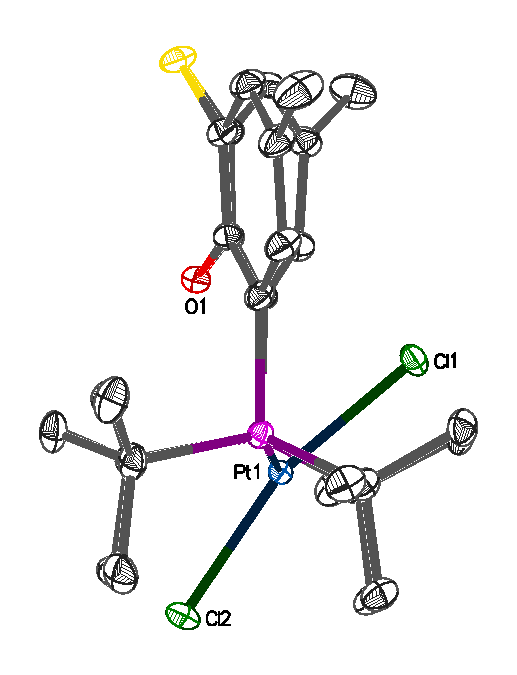
\includegraphics[scale=0.8]{../Figures/Crystalthixantphosplatinumdichlorideside.eps}
\caption[X-ray crystal structure of \ce{[Pt(\tButhixantphos)Cl2]}, side view]{X-ray crystal structure of \ce{[Pt(\tButhixantphos)Cl2]}, side view}
\vspace{0.2cm}
\label{crystalthixantphosplatinumdichlorideside}
\end{center}
\end{figure}
\vspace{0.2cm}

\begin{table}[ht]
\caption[Selected bond distances (\AA) and angles (\degrees) of \ce{[Pt(\tButhixantphos)Cl2]}]{Selected bond distances (\AA) and angles (\degrees) of \ce{[Pt(\tButhixantphos)Cl2]}}
\vspace{1em}
\label{table:crystalthixantphosplatinumdichloride:lengths}
\small
\begin{center}
\begin{tabular}{l l l l}
	\toprule
	\multicolumn{2}{l}{\bfseries{~Bond distances (\si{\angstrom})}} & \multicolumn{2}{c}{\bfseries{Bond angles (\degrees)}} \\
	\midrule		
	~P1-P2		~~&~~4.5037(6)~~	&~~P1-Pt-P2			&~~116.68(3)~~	\\	
	~P1-Pt		~~&~~2.3205(4)~~	&~~Cl1-Pt-Cl2			&~~164.235(15)~~	\\
	~P2-Pt		~~&~~2.3239(4)~~	&~~P1-Pt-Cl1			&~~87.11(15)~~	\\
	~Pt-Cl1		~~&~~2.3209(4)~~	&~~P1-Pt-Cl2			&~~95.939(16)~~	\\
	~Pt-Cl2		~~&~~2.3098(4)~~	&~~P2-Pt-Cl1			&~~86.699(14)~~	\\
	~Pt...O		~~&~~2.8016(11)~~	&~~P2-Pt-Cl2			&~~96.917(15)~~	\\
	~				&			&~~Ring 1-Ring 2		&~~139.11(6)~~	\\
	\bottomrule{}
\end{tabular}
\end{center}
\end{table}

\begin{table}[htp]
\small
\caption[Crystallographic Data and Structure Refinement of \ce{[Pt(\tButhixantphos)Cl2]}]{Crystallographic Data and Structure Refinement of \ce{[Pt(\tButhixantphos)Cl2]}} 
\vspace{1em}
\label{table:crystalthixantphosplatinumdichloride:data}
\small
\begin{center}
\begin{tabular}{l l}
	\toprule
	\bfseries{Empirical formula}~~& \bfseries{\ce{C30H46Cl2OP2PtS}}\\
	\midrule
	Formula weight	 							& 782.66\\
	Temperature/K	 							& 284.87(10)\\
	Crystal system	 							& monoclinic\\
	Space group	 							& P2\sub{1}/c\\
	a$/$\si{\angstrom}							& 15.26769(8)\\
	b$/$\si{\angstrom} 							& 10.98650(7)\\
	c$/$\si{\angstrom}							& 19.05134(13)\\
	$\alpha/$\degrees							& 90\\
	$\beta/$\degrees							& 95.2318(5)\\
	$\gamma/$\degrees							& 90\\
	Volume$/$\si{\angstrom\cubed}  				& 3182.33(3)\\
	Z	 									& 4\\
$\rho$\sub{calc} \si{\milli\gram}$/$\si{\milli\metre\cubed} 	& 1.634\\
\si{\metre}$/$\si{\milli\metre} 						& 4.766\\
F(000)	 									& 1568.0\\
Crystal size$/$\si{\milli\metre\cubed}	 				& 0.27 x 0.14 x 0.08\\
Radiation	 									& MoK$\alpha$ ($\lambda$ = 0.71073)\\
2$\theta$ range for data collection					& 5.264 to 75.522\degrees\\
Index ranges	 								& -25 $\leq$ h $\leq$ 25, -15 $\leq$ k $\leq$ 18, -32 $\leq$ l $\leq$ 31\\
Reflections collected	 							& 49341\\
Independent reflections	 						& 16242 [R\sub{int} = 0.0277, R\sub{sigma} = 0.0333]\\
Data$/$restraints$/$parameters					& 16242$/$0$/$348\\
Goodness-of-fit on F$^{2}$	 					& 1.076\\
Final R indexes [I$>$=2$\sigma$ (I)]	 				& R\sub{1} = 0.0240, wR\sub{2} = 0.0445\\
Final R indexes [all data]	 						& R\sub{1} = 0.0351, wR\sub{2} = 0.0486\\
Largest diff. peak/hole / e \si{\per\angstrom\cubed}		& 1.46/-1.27	\\
	\bottomrule
\end{tabular}
\end{center}
\end{table}

Although a vast number of platinum dichloride starting materials were investigated the reactions were generally carried out in CDCl3 so they mostly just formed the protonated ligand.  However it looks like PtCl2(tBuCN) reacted with the protonated ligand that formed - maybe worth trying this again in something like benzene or acetone. 

In order to test the chloride dissociation theory we dissolved the complex in acetone and reacted with ammonium hexafluorophosphate.  The solution changed over 30 minutes from deep orange to yellow and a precipitate of ammonium chloride formed.  The product appeared at 46.4 ppm (\JPtP = 2347 Hz) in the \phosphorus{} NMR spectrum with an associate septet at -144.5 ppm indicative of \ce{PF6}.  The platinum phosphorus coupling constant had dropped from the dichloride complex by 353 Hz.  This indicates that the phosphorus atoms are still in a trans configuration but they are more strongly bound to the platinum \fixme{?}  As the platinum has lost a chloride ligand it will have less electron density and thus will bond more strongly to the phosphines to compensate.  A shift in the \carbon{} NMR spectrum for the carbon adjacent to the ether bridge also occurred from 155.8 ppm to 157.4 ppm.  This downfield  shift is indicative of a deshielding of the carbon centre.  This deshielding may be the result of oxygen coordination as the oxygen donates electron density to the platinum it will pull electron density from the surrounding carbons resulting in deshielding of those carbons.  The \carbon{} NMR resonance for the aromatic carbon \emph{ipso} to phosphorus has shifted significantly upfield from 124.5 to 119.1 ppm.\fixme{why?}

The relationship between these two compounds was further studied by variable temperature \phosphorus NMR analysis \fixme{figure?}.  A sample of \ce{[Pt(tBu-thixantphos)Cl2]} in \ce{CD2Cl2} was analysed down to -80 \degC.  At room temperature a single broad resonance at 32.9 ppm was observed.  Upon cooling down to -20 \degC this resolved into a single sharp peak, however cooling further led to the conversion of this dichloride into the monochloride appearing at 46.4 ppm.  The mono chloride became the major product below approx -60 \degC.  This may be due to the steric influence of the chlorides and the diphosphine.  At room temperature and above the complex has sufficient energy to exchange between the dichloride and monochloride complexes resulting in a single broad peak.  However upon lowering the temperature the dichloride is preferred.  Lowering further preferences the monochloride.  This effect is likely sterics, at the lower temperature the complex has less energy to move and thus prefers a structure with sufficient space to for all of the ligands around the platinum.  

\subsubsection{Reactions of Pt(POP)Cl}

Hybrid ligands have attracted attention recently due to their combination of different bonding atoms which can lead to differing activity in the trans positions.  If one of the ligating atoms is a weak donor group then the ligand can also exhibit hemilability where the weakly bonding ligand can be displaced by something else (such as a reagent in a catalytic reaction) but the ligand still remains anchored to the metal centre and can thus still influence the reaction and can recoordinate rapidly once the reaction is complete thus stabilising the resting state for the catalyst.  

The complex \ce{[Pt(POP)Cl]PF6} where POP = tBu-thixantphos bonding through the two phosphines and the oxygen.  Has the potential for hemilability of the ether bridge.  This was investigated by reaction with carbon monoxide (Scheme \fixme{draw a scheme}).  The first complex is as expected where the carbon monoxide displaces the oxygen and coordinates to the platinum centre.  However, this then reacts (most likely with adventitious water) to displace the chloride and form a hydride complex.  This complex is only stable under an excess of carbon monoxide and readily loses CO and the oxygen recoordinates thus demonstrating hemilability.  Using \carbon{} enriched carbon monoxide allowed for further characterisation.  Selected NMR data for these compounds are summarised in Table \fixme{put a table here}.

\subsection{Reactions with platinum dimethyl starting materials}

Metal alkyl complexes form as intermediates in a wide range of catalytic transformations including polymerisation reactions and C-H activation.  If methane underwent C-H activation on a platinum centre then a platinum methyl complex would be formed.  These complexes are also interesting for their potential protonation to form a sigma-methane complexes similar to that reported by Brookhart.\cite{Bernskoetter2009}  

tBu-Thixantphos was reacted with \ce{[Pt(hex)Me2]} in a benzene solution.  Even with high temperatures \fixme{check what they were} and extended reaction times no reaction was observed.  An equivalent of acid was added to attempt to promote loss of methane and coordination of the diphosphine, however the acid reacted exclusively with the diphosphine instead of \ce{[Pt(hex)Me2]}.  In order to form a complex, Initial reaction between the diphosphine and \ce{[Pt(hex)Me2]} may form a complex with a dimethyl and a monodentate phosphine and hexadiene (Scheme \ref{scheme:dimethyl}).  If this forms then the steric bulk resulting from two bidentate ligands in monodentate coordination may destabilise the complex thus favouring loss of the monodentate phosphine to reform the starting materials rather than rearrangement of the strongly bound methyls into a trans configuration.

\begin{scheme}[ht]
\begin{center}
\vspace{0.5cm}
\includegraphics{../Schemes/Dimethyl.eps}
\caption[Proposed reaction between \ce{[Pt(hex)Me2]} and a diphosphine ligand]{Proposed reaction between \ce{[Pt(hex)Me2]} and a tBu-xantphos diphosphine ligand (abbreviated PP)}
\vspace{0.2cm}
\label{scheme:dimethyl}
\end{center}
\end{scheme}
\vspace{0.2cm}

\subsection{Reactions with platinum chloro methyl starting materials}

Reaction with \ce{[Pt(hex)ClMe]} is much faster than either the \ce{[Pt(hex)Cl2]} or \ce{[Pt(hex)Me2]}.  This may be due to the faster reorganisation to a \emph{trans} geometry as a result of the stronger \emph{trans} influence of the methyl to promote loss of the chloride.  A single product is observed as a single sharp peak in \ce{d6-acetone} at 50.5 ppm (\JPtP{} = 2793 Hz).  This indicates \emph{trans}-coordination of the diphosphine.  Contrary to the reaction with \ce{[Pt(hex)Cl2]}, the complex that forms exclusively is a tridentate methyl complex (Scheme \ref{scheme:platinumchloromethyl}).  Due to the high \emph{trans} influence of the methyl the loss of the chloride is promoted and this is the only product even without the addition of \ce{NH4PF6} to promote the reaction.  

\begin{scheme}[ht]
\begin{center}
\vspace{0.5cm}
\includegraphics{../Schemes/Platinumchloromethyl.eps}
\caption[Reaction between \ce{[Pt(hex)ClMe]} and tBu-thixantphos]{Reaction between \ce{[Pt(hex)ClMe]} and tBu-thixantphos}
\vspace{0.2cm}
\label{scheme:platinumchloromethyl}
\end{center}
\end{scheme}
\vspace{0.2cm}

The platinum methyl appears in the \proton{} NMR spectrum at 1.94 ppm as a triplet (coupling to both phosphorus atoms) with platinum satellites of 97.4 Hz.  This is very large for a two-bond platinum coupling and is indicative of a very weakly bound group \emph{trans} to the methyl.  Similar complexes reported previously include \fixme{reference ingleson2004 and others?} which have similar platinum couplings.  However the resonance for the methyl in the \carbon{} NMR spectrum is present at -23.8 ppm as a triplet with platinum satellites of 777.2 Hz.  To the best of our knowledge this is the largest reported platinum coupling constant to a methyl carbon.  All of this data supports the structure proposed as not having an interaction between the oxygen and the platinum.  Although there may be one present it is very weakly bound.  The most similar NMR data has platinum methyls \emph{trans} to weakly bound agostic interactions of isopropyl or t-butyl groups.  In these cases no evidence of the agostic interaction was seen in the NMR spectra it was only observed in the X-ray crystal structure.  Low temperature NMR down to -80~\degC{} showed no evidence for an agostic interaction.  It is also likely that as t-Bu thixantphos has an oxygen present close to the platinum that this would coordinate preferentially to forming an agostic.  


\begin{sidewaystable}[ht]
\caption[Selected NMR Data for Platinum Methyl complexes with Xantphos Ligands]{Selected NMR Data for Platinum Methyl complexes with Xantphos Ligands in \ce{d6-acetone}}
\vspace{1em}
\label{table:platinummethyls}
\small
\begin{center}
\begin{tabular}{l c c c c c}
	\toprule
	~ & \multicolumn{2}{c}{\bfseries{\phosphorus}} & \bfseries{\proton} & \multicolumn{2}{c}{\bfseries{\carbon}} \\
	\cmidrule(lr){2-3} \cmidrule(lr){4-4} \cmidrule(lr){5-6} 
	~\bfseries{Diphosphine} & \bfseries{$\delta/$ppm} &\bfseries{$\Delta\delta/$ppm}&\bfseries{\ce{Pt-CH3} $\delta/$ppm} & \bfseries{\ce{Pt-CH3} $\delta/$ppm} & \bfseries{$\Delta \delta$ C-O $/$ppm} \\
	\midrule		
	~\tBuXantphos{}	& 51.0 (2788) & 40.8 & 1.92 (97.4) & -23.9 (774.6) & 0.3\\
	~\tBuThixantphos	& 50.5 (2793) & 41.0 &1.94 (97.4) & -23.8 (777.2) & -1.5\\
	~\tBuSixantphos	& 48.7 (2763) & 40.3 & 2.01 (98.6) & -22.7 (780.5) & 3.0\\
	\bottomrule{}
\end{tabular}
\end{center}
\end{sidewaystable}

%Delta deltas are given as coordinated -free

\fixme{make sure that all of this is good}  

\section{Reaction with palladium(II) precursors}

The work with palladium(II) precursors is similar to that with platinum(II).  Palladium dichloride complexes are widely used as precatalysts for a large number of different catalytic transformations.\fixme{citation}  \ce{[Pd(COD)Cl2]} was used as the palladium precusor as it is the most commonly used starting material for the synthesis of palladium dichloride complexes.  

Reaction between the tBu-xantphos ligands and \ce{[Pd(COD)Cl2]} was much faster than with any of the platinum dichloride analogues with a dark red species forming rapidly.  A single complex was observed in all cases with single peaks observed in each of the phosphorus NMR spectra.\fixme{give values}  This indicates a symmetrical complex has formed, the \emph{tert}-butyl peaks in the \proton{} NMR spectrum appear as a virtual triplet resonance indicative of \emph{trans}-chelation (Scheme \ref{Palladiumdichloride}).  

\begin{scheme}[ht]
\begin{center}
\vspace{0.5cm}
\includegraphics{../Schemes/Palladiumdichloride.eps}
\caption[Reaction between \ce{[Pd(COD)Cl2]} and tBu-thixantphos]{Reaction between \ce{[Pd(COD)Cl2]} and tBu-xantphos ligands}
\vspace{0.2cm}
\label{Palladiumdichloride}
\end{center}
\end{scheme}
\vspace{0.2cm}

The chloride ligands in \ce{[Pd(tBu-xantphos)Cl2]} are relatively weakly, similarly to the platinum case, however no evidence for a monochloride complex is apparent.  Reacting the dichloride complexes with \ce{NH4PF6} in acetone forms an immediate precipitate of \ce{NH4Cl} and the reaction colour changes from a deep red to yellow.\fixme{check that this isn't for the platinum one}  The product has two peaks in the \phosphorus{} NMR spectrum, a septet at -144.5 (710.5 Hz) and a singlet at 56.4 ppm (shifted from 41.9 ppm) indicative of a symmetrical complex and a virtual triplet resonance for the \emph{tert}-butyl peaks.  The O-ipso carbon has a insignificant shift in the \carbon{} NMR spectrum (from 155.1 to 154.9 ppm) indicating that it is likely not coordinated to the palladium.  A large shift occurs for the P-ipso carbon shifting from 123.5 (vt, 12.5 Hz) to 118.7 (vt, 10.8 Hz).  This indicates an increase in the electron density on the carbon and is close to that found for the complex \ce{[Ag(tBu-xantphos)Cl]} (120.9 ppm).  This data confirms the formulation of the complex as \ce{[Pd($\eta^2-$(tBu-xantphos)Cl]PF6}

